\documentclass[conference]{IEEEtran}

% ── Fontes ────────────────────────────────────────────────────────────────────
\usepackage{fontspec}
\defaultfontfeatures{Ligatures=TeX}
\setmainfont{TeX Gyre Termes}
\setmonofont[Scale=0.86]{Latin Modern Mono}
\usepackage{microtype}

% ── Matemática ────────────────────────────────────────────────────────────────
\usepackage{amsmath, amssymb}

% ── Figuras e tabelas ─────────────────────────────────────────────────────────
\usepackage{graphicx}
\graphicspath{{reports/figures/}}
\usepackage{booktabs}
\usepackage{array}
\usepackage[caption=false,font=footnotesize]{subfig}

% ── Código ────────────────────────────────────────────────────────────────────
\usepackage{listings}
\usepackage{xcolor}

% ── Citações e links ──────────────────────────────────────────────────────────
\usepackage{cite}
\usepackage{url}
\usepackage[hidelinks]{hyperref}

\definecolor{codebg}{RGB}{250,250,250}
\definecolor{codegreen}{RGB}{40,120,40}
\definecolor{codeblue}{RGB}{0,60,180}
\definecolor{codeorange}{RGB}{180,60,0}
\definecolor{codegray}{RGB}{130,130,130}

\lstdefinestyle{python}{
  language=Python,
  backgroundcolor=\color{codebg},
  commentstyle=\color{codegreen}\itshape,
  keywordstyle=\color{codeblue}\bfseries,
  stringstyle=\color{codeorange},
  numberstyle=\tiny\color{codegray},
  basicstyle=\ttfamily\footnotesize,
  breaklines=true,
  captionpos=b,
  numbers=left,
  numbersep=6pt,
  showstringspaces=false,
  tabsize=4,
  frame=single,
  rulecolor=\color{codegray!40},
  xleftmargin=1.5em,
  aboveskip=8pt,
  belowskip=4pt,
}
\lstset{style=python}

% ── Auxiliares ────────────────────────────────────────────────────────────────
\newcommand{\fonte}[1][elaborado pelos autores.]{%
  \par\vspace{1pt}{\footnotesize\centering Fonte: #1\par}}
\newcommand{\instituicao}{Universidade Federal de São Paulo — UNIFESP}
\newcommand{\disciplina}{Inteligência Artificial}
\newcommand{\cidade}{São José dos Campos}

\title{Predição e Classificação de Risco de Burnout\\\large Pipeline de Aprendizado de Máquina Aplicado à Gestão de Saúde Ocupacional}

\author{%
\IEEEauthorblockN{Breno Porto Pinheiro do Prado, RA 185196\\Guilherme Bento Ramos, RA 185226}
\IEEEauthorblockA{\instituicao\\
\cidade\\
2026}
}

% ─────────────────────────────────────────────────────────────────────────────
\begin{document}
% ─────────────────────────────────────────────────────────────────────────────

\maketitle

\begin{abstract}
	O esgotamento profissional (\textit{burnout}) configura crescente desafio de
	saúde ocupacional com impactos documentados sobre produtividade,
	rotatividade e bem-estar. Este trabalho propõe um \textit{pipeline} modular
	de aprendizado de máquina para predição e classificação de risco de
	\textit{burnout}, alinhado aos Objetivos de Desenvolvimento Sustentável
	ODS~3, ODS~8 e ODS~10 da ONU. A partir do \textit{dataset}
	\textit{``Remote Work Health Impact Survey 2025''} (Kaggle, 3.157
	registros, coletado em junho de 2025), o sistema percorre cinco etapas:
	Análise exploratória, pré-processamento sem vazamento de dados,
	treinamento comparativo de Regressão Linear, Random Forest e XGBoost,
	avaliação com K-Fold e análise de equidade, e função de
	\textit{scoring} individual. O alvo \texttt{Burnout\_Level}
	(categórico ordinal: Low, Medium, High) é tratado como regressão ordinal,
	com \textit{score} normalizado para $[0,1]$. Os três modelos alcançaram
	desempenho similar sobre os dados de survey auto-reportados
	(R²\,$\approx$\,0,04; MAE\,$\approx$\,0,64 na escala ordinal 0--2).
	A \textit{feature} mais influente na Regressão Linear foi
	\texttt{Work\_Arrangement} ($w=+0{,}364$), enquanto o Random Forest
	distribuiu importância entre \texttt{Age} (16,5\%),
	\texttt{Hours\_Per\_Week} (15,3\%) e \texttt{Job\_Role} (13,4\%).
	Achado relevante da EDA: trabalhadores em regime \textit{remote}
	apresentam burnout médio superior ao regime presencial
	(1,33 vs.\ 0,96 na escala ordinal).
\end{abstract}

\begin{IEEEkeywords}
	burnout, aprendizado de máquina, regressão, XGBoost, Random Forest, saúde ocupacional, \textit{scoring} de risco, ODS
\end{IEEEkeywords}

% ═════════════════════════════════════════════════════════════════════════════
\section{Introdução}
\label{sec:intro}
% ═════════════════════════════════════════════════════════════════════════════

O esgotamento profissional (\textit{burnout}) é um fenômeno psicossocial de
impacto crescente nas organizações contemporâneas. Definido por Maslach e
Jackson \cite{maslach1981} como síndrome de exaustão emocional,
despersonalização e redução do senso de realização pessoal, o
\textit{burnout} foi reconhecido em 2019 pela Organização Mundial da Saúde
(OMS) como fenômeno ocupacional na Classificação Internacional de Doenças
(CID-11). Pesquisas de longo prazo associam o fenômeno a absenteísmo
elevado, intenção de abandono de cargo, doenças cardiovasculares e
transtornos mentais \cite{salvagioni2017}.

A relevância do tema transcende o âmbito individual: o esgotamento de
trabalhadores impõe custos sistêmicos à saúde pública e à economia.
Nesse sentido, este trabalho está alinhado a três Objetivos de
Desenvolvimento Sustentável da ONU \cite{onu_ods}:

\begin{itemize}
	\item \textbf{ODS 3 — Saúde e Bem-Estar:} promoção de ambientes de
	      trabalho saudáveis e redução de agravos à saúde mental;
	\item \textbf{ODS 8 — Trabalho Decente e Crescimento Econômico:}
	      proteção dos direitos trabalhistas e condições de trabalho
	      seguras e saudáveis para todos;
	\item \textbf{ODS 10 — Redução das Desigualdades:} identificação de
	      subgrupos com maior exposição ao risco para permitir intervenções
	      equitativas.
\end{itemize}

A detecção precoce do risco de \textit{burnout} é substancialmente mais
eficaz do que estratégias reativas. Técnicas de aprendizado de máquina
permitem identificar padrões de risco a partir de dados de recursos humanos
já coletados pelas organizações — como carga de trabalho alocada, nível de
fadiga mental e tempo de empresa — sem a necessidade de instrumentos
psicométricos adicionais.

É fundamental, contudo, delimitar o escopo do sistema: o \textit{pipeline}
proposto é uma \textbf{ferramenta de triagem estatística}, não um
instrumento de diagnóstico clínico. O escore produzido indica a
\textit{probabilidade estimada} de esgotamento com base em padrões
históricos observados nos dados de treinamento. A interpretação do
resultado e qualquer decisão sobre intervenção devem envolver profissionais
de saúde habilitados (psicólogo, médico do trabalho) e a equipe de RH.

Este trabalho constrói um \textit{pipeline} modular, com código aberto e
reprodutível (SEED\,=\,42), que compara três modelos de regressão em
complexidade crescente, avalia equidade preditiva por subgrupos e entrega
um script interativo de \textit{scoring} individual em terminal. O documento está
organizado da seguinte forma: a Seção~\ref{sec:dataset} descreve o
\textit{dataset}; a Seção~\ref{sec:pipeline} apresenta a arquitetura do
\textit{pipeline}; as Seções~\ref{sec:eda}–\ref{sec:scoring_sec} detalham
cada etapa; a Seção~\ref{sec:eval} apresenta os resultados; a
Seção~\ref{sec:equity} discute equidade; e as Seções~\ref{sec:limit}
e~\ref{sec:conc} encerram com limitações e conclusão.

% ═════════════════════════════════════════════════════════════════════════════
\section{Dataset}
\label{sec:dataset}
% ═════════════════════════════════════════════════════════════════════════════

\subsection{Descrição}

O \textit{dataset} \textit{``Remote Work Health Impact Survey 2025''}
\cite{kaggle_dataset}, disponível publicamente na plataforma Kaggle,
reúne respostas de um survey global aplicado em junho de 2025 a
trabalhadores em regimes remoto, híbrido e presencial no período
pós-pandemia. O conjunto possui \textbf{3.157 registros} e
\textbf{14 colunas} (Tabela~\ref{tab:features}). A variável alvo,
\texttt{Burnout\_Level}, é categórica ordinal com três categorias:
\texttt{Low}, \texttt{Medium} e \texttt{High}, que foram convertidas
para representação numérica (0, 1 e 2) tratada como regressão ordinal.
A distribuição do alvo é: Low = 23,6\%, Medium = 43,3\%,
High = 33,1\%. Nenhuma linha apresenta alvo ausente.

\begin{table*}[!t]
	\centering
	\small
	\setlength{\tabcolsep}{4pt}
	\caption{Variáveis do \textit{dataset} \textit{``Remote Work Health Impact Survey 2025''}.}
	\label{tab:features}
	\begin{tabular}{lllc}
		\toprule
		\textbf{Coluna}            & \textbf{Tipo}     & \textbf{Faixa / Valores}         & \textbf{Papel}                      \\
		\midrule
		Survey\_Date               & Data              & Junho/2025                       & Descartada                          \\
		Age                        & Num.\ inteira     & 22--65                           & Feature                             \\
		Gender                     & Categ.\ nominal   & Female, Male, Non-binary, \ldots & Feature                             \\
		Region                     & Categ.\ nominal   & 6 regiões globais                & Feature                             \\
		Industry                   & Categ.\ nominal   & 9 setores                        & Feature                             \\
		Job\_Role                  & Categ.\ nominal   & 24 cargos                        & Feature                             \\
		Work\_Arrangement          & Categ.\ ordinal   & Onsite, Hybrid, Remote           & Feature                             \\
		Hours\_Per\_Week           & Num.\ inteira     & 35--65                           & Feature                             \\
		Mental\_Health\_Status     & Categ.\ nominal   & 6 condições + None               & Feature                             \\
		\textbf{Burnout\_Level}    & Categ.\ ordinal   & Low, Medium, High                & \textbf{Alvo}                       \\
		Work\_Life\_Balance\_Score & Num.\ ordinal     & 1--5                             & Feature                             \\
		Physical\_Health\_Issues   & Texto multi-label & var.\ ou ausente                 & $\to$ \texttt{has\_physical\_issue} \\
		Social\_Isolation\_Score   & Num.\ ordinal     & 1--5                             & Feature                             \\
		Salary\_Range              & Categ.\ ordinal   & \$40K--\$120K+                   & Feature                             \\
		\bottomrule
	\end{tabular}
	\fonte
\end{table*}

As únicas colunas com valores ausentes são
\texttt{Mental\_Health\_Status} (799 registros, 25,3\%) e
\texttt{Physical\_Health\_Issues} (280 registros, 8,9\%).
O alvo \texttt{Burnout\_Level} não apresenta valores ausentes.

\subsection{Natureza e Contexto do Dataset}

O \textit{dataset} \textit{``Remote Work Health Impact Survey 2025''}
\cite{kaggle_dataset} foi coletado em junho de 2025 e representa uma
amostra global de trabalhadores em regime remoto, híbrido e presencial
no período pós-pandemia. Os dados são auto-reportados por meio de
survey anônimo, cobrindo 3.157 respondentes de múltiplas
regiões, setores e faixas etárias. O uso de dados reais de survey
--- em contraste com datasets sintéticos --- confere maior validade
ecológica às conclusões, embora introduza viés de resposta e
seleção amostral inerentes à metodologia de survey.
O campo \texttt{Survey\_Date} é uniforme em junho de 2025 e foi
descartado por não agregar sinal preditivo direto ao modelo.

Esse conjunto é apropriado para este trabalho porque possui variável-alvo
clara, atributos plausíveis, acesso público e licença aberta.
O impacto das limitações é discutido na Seção~\ref{sec:limit}.

% ═════════════════════════════════════════════════════════════════════════════
\section{Arquitetura do Pipeline}
\label{sec:pipeline}
% ═════════════════════════════════════════════════════════════════════════════

O sistema é estruturado como um \textit{pipeline} sequencial de cinco
etapas, cada uma implementada em um módulo Python dedicado
(Tabela~\ref{tab:pipeline}). A modularidade garante que cada componente
possa ser executado, testado e atualizado de forma independente.

\begin{table*}[!t]
	\centering
	\caption{Componentes do pipeline e respectivos módulos.}
	\label{tab:pipeline}
	\begin{tabular}{clll}
		\toprule
		\textbf{Etapa} & \textbf{Módulo}                         & \textbf{Responsabilidade} & \textbf{Saídas} \\
		\midrule
		1              & \texttt{src/eda.py}
		               & Análise exploratória
		               & 5 gráficos em \texttt{reports/figures/}                                               \\
		2              & \texttt{src/preprocessing.py}
		               & Limpeza e transformação
		               & CSVs processados + \texttt{.pkl}                                                      \\
		3              & \texttt{src/training.py}
		               & Treinamento dos modelos
		               & 3 modelos em \texttt{models/}                                                         \\
		4              & \texttt{src/evaluation.py}
		               & Avaliação e comparação
		               & Tabelas + gráficos de resultado                                                       \\
		5              & \texttt{src/scoring.py}
		               & Scoring individual
		               & Função \texttt{predict\_burnout()}                                                    \\
		\bottomrule
	\end{tabular}
	\fonte
\end{table*}

O fluxo de dados segue estritamente a ordem das etapas: a EDA informa as
decisões de pré-processamento; o pré-processamento produz os dados limpos
e os artefatos de transformação (\texttt{imputer.pkl},
\texttt{scaler.pkl}); o treinamento produz os modelos serializados
(\texttt{.pkl}); a avaliação consome todos os artefatos anteriores para
medir o desempenho; e o \textit{scoring} reutiliza os artefatos de
transformação e o melhor modelo para predições em tempo real.

A reprodutibilidade é garantida por dois parâmetros globais definidos em
\texttt{src/config.py} e utilizados em todos os componentes:

\begin{itemize}
	\item \texttt{SEED\,=\,42} — semente fixa aplicada na divisão
	      treino/teste (\texttt{train\_test\_split}), no Random Forest
	      (\texttt{random\_state}), no XGBoost e no K-Fold. Qualquer
	      execução do \textit{pipeline} com os mesmos dados produz
	      exatamente os mesmos resultados.
\end{itemize}

% ═════════════════════════════════════════════════════════════════════════════
\section{Etapa 1 — Análise Exploratória dos Dados}
\label{sec:eda}
% ═════════════════════════════════════════════════════════════════════════════

\subsection{Distribuição da variável alvo}

O \texttt{Burnout\_Level} é distribuído em três categorias: \textbf{Low}
(23,6\%), \textbf{Medium} (43,3\%) e \textbf{High} (33,1\%)
(Figura~\ref{fig:dist}). A maior concentração em ``Medium'' indica
que a maioria dos respondentes auto-relata nível moderado de esgotamento.

\begin{figure*}[!t]
	\centering
	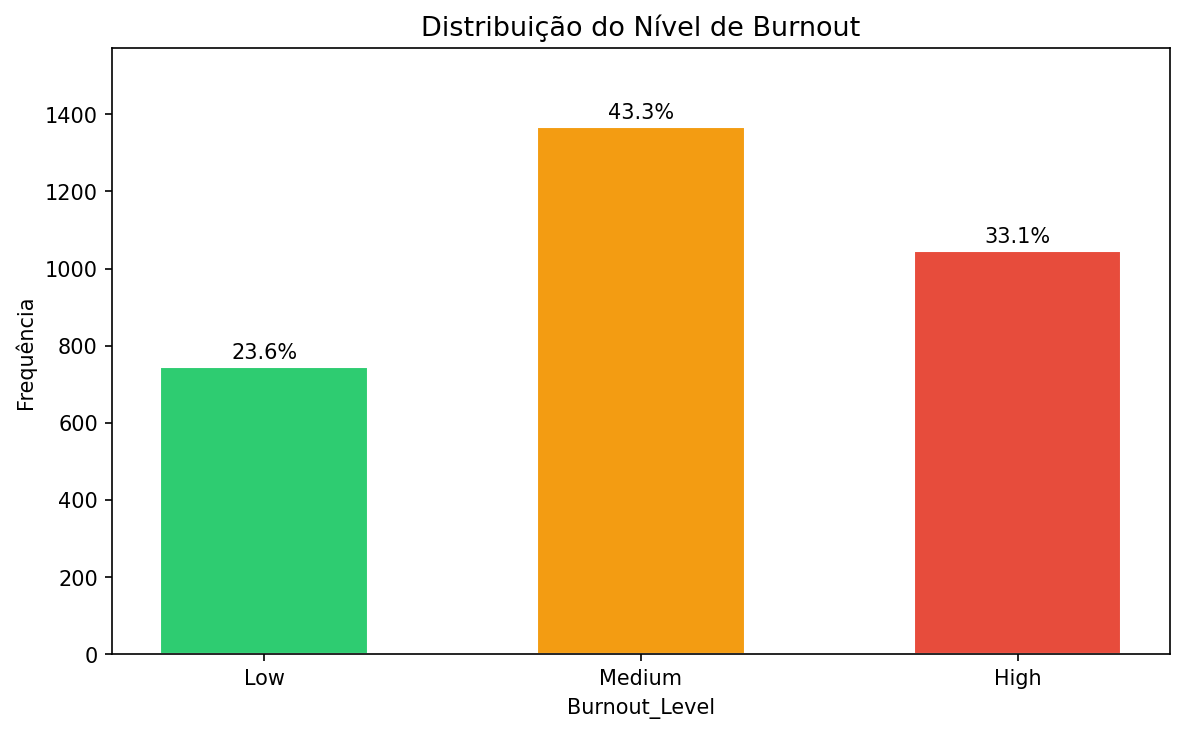
\includegraphics[width=0.99\textwidth,height=0.32\textheight,keepaspectratio]{burnout_distribution.png}
	\caption{Distribuição da variável alvo \texttt{Burnout\_Level} (barras por categoria).}
	\fonte
	\label{fig:dist}
\end{figure*}

\subsection{Correlações e achado principal}

O mapa de calor de correlação de Pearson (Figura~\ref{fig:heat}) mostra
correlações fracas entre as variáveis numéricas e o alvo --- esperado em
dados de survey auto-reportados. A correlação mais forte com
\texttt{Burnout\_Level} (codificado como 0--2) é a de
\texttt{Social\_Isolation\_Score} (+0,044). \texttt{Work\_Life\_Balance\_Score}
apresenta correlação levemente negativa (--0,018), sugerindo que melhor
equílíbrio vida-trabalho se associa a menos burnout. Horas semanais e
idade têm correlações praticamente nulas.

\begin{figure*}[!t]
	\centering
	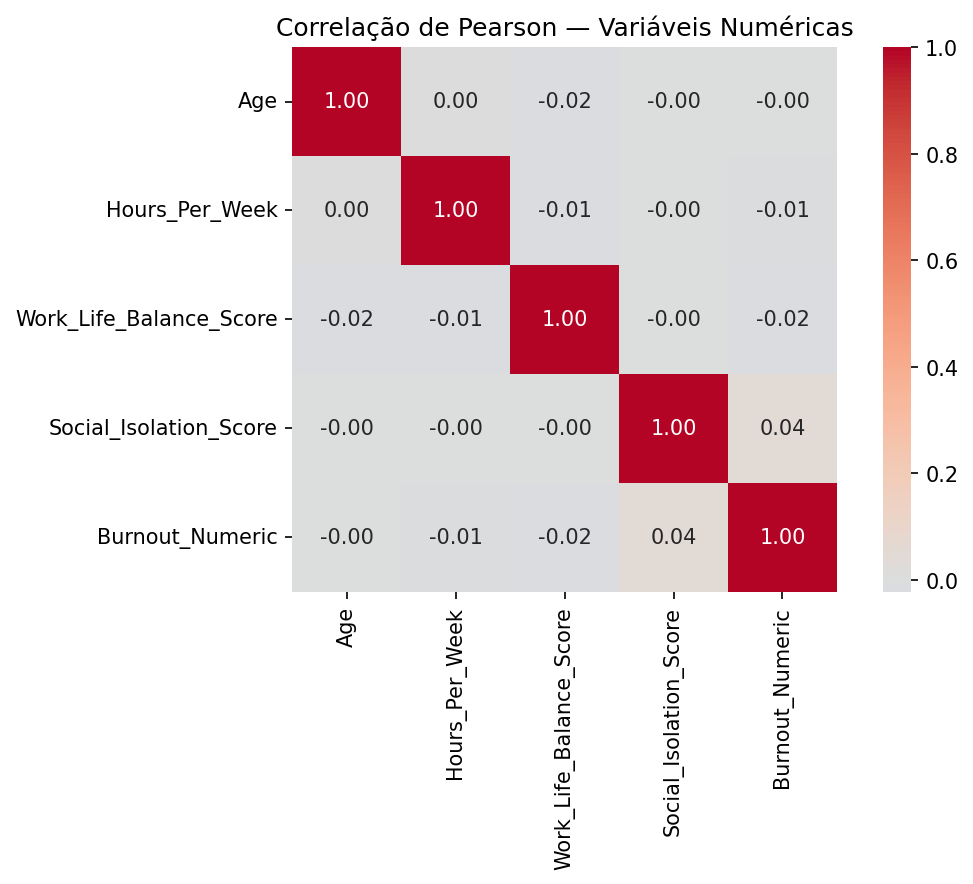
\includegraphics[width=0.99\textwidth,height=0.32\textheight,keepaspectratio]{correlation_heatmap.png}
	\caption{Mapa de calor de correlação de Pearson entre variáveis numéricas.}
	\fonte
	\label{fig:heat}
\end{figure*}

\subsection{Análise por subgrupos}

A Figura~\ref{fig:subgroups} apresenta a distribuição do
\texttt{Burnout\_Level} segmentada pelas variáveis de regime de
trabalho, gênero e setor. Os achados principais são:

\begin{itemize}
	\item \textbf{Regime de trabalho:} trabalhadores em regime
	      \textit{remote} apresentam burnout médio de 1,33 (escala 0--2),
	      superior ao regime híbrido (1,17) e presencial (0,96). O regime
	      remoto associa-se, neste dataset, ao \textbf{maior} nível de
	      esgotamento --- achado contraintuitivo que reflete possivelmente
	      maior isolamento social reportado por trabalhadores remotos;
	\item \textbf{Gênero:} as diferenças entre gêneros são pequenas
	      (variação $<$\,2 p.p.\ em burnout alto), sem subgrupo
	      sistematicamente mais afetado;
	\item \textbf{Setor:} a prevalência de burnout alto varia entre
	      setores, com \textit{Customer Service} e \textit{Manufacturing}
	      entre os mais afetados.
\end{itemize}

\begin{figure*}[!t]
	\centering
	\subfloat[Por regime de trabalho]{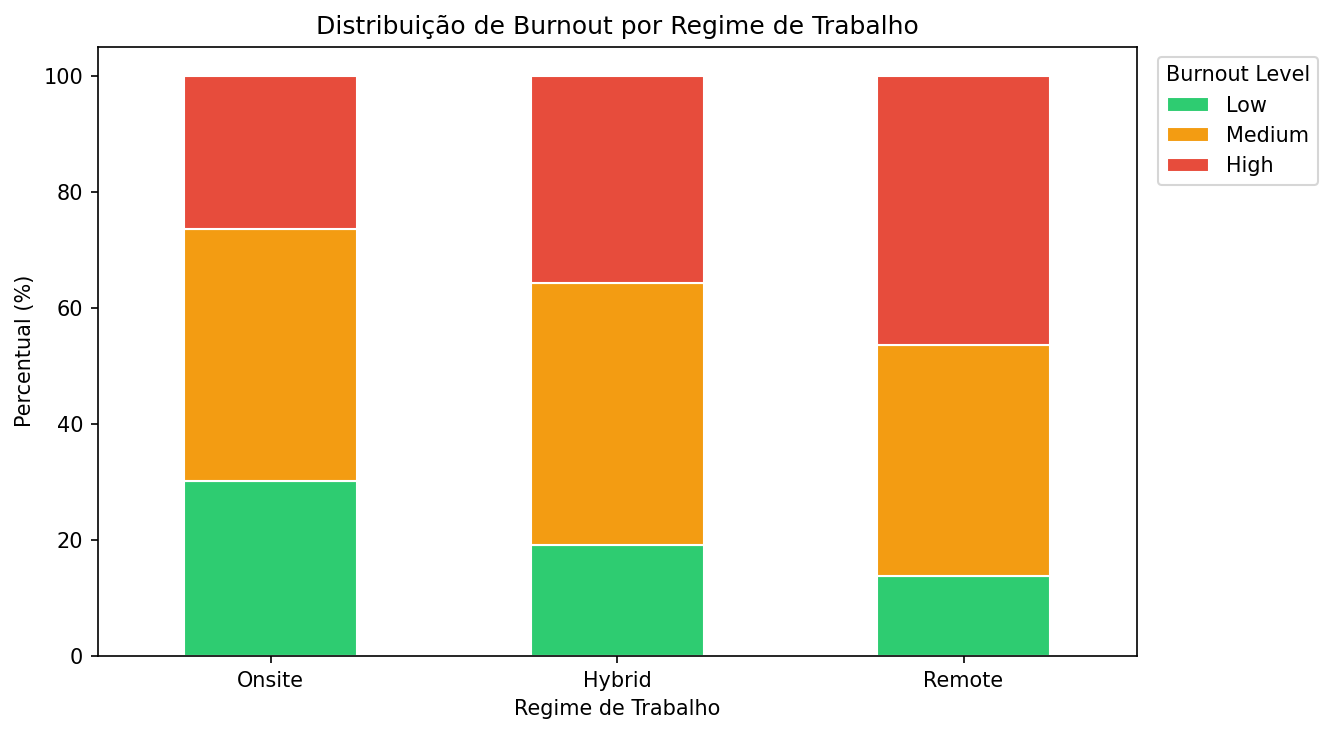
\includegraphics[width=0.49\textwidth,height=0.26\textheight,keepaspectratio]{burnout_by_work_location.png}}\hfill
	\subfloat[Por gênero]{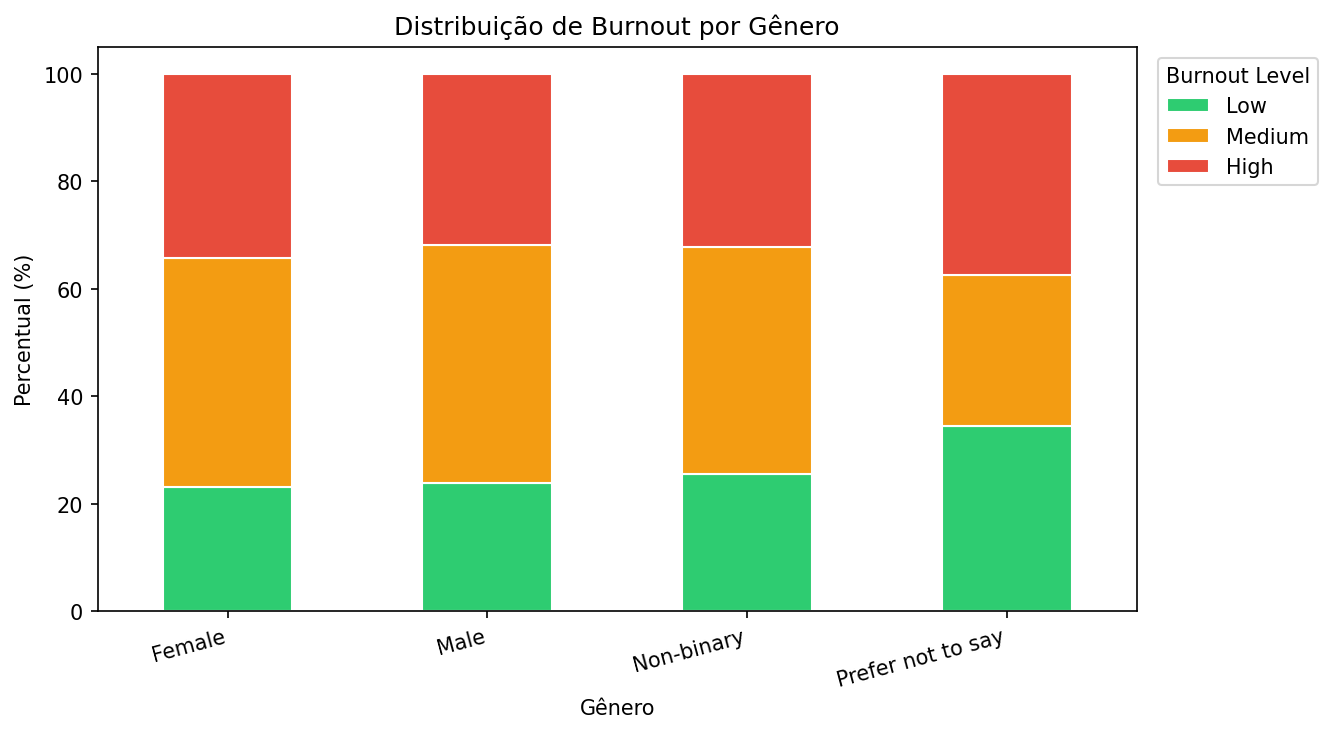
\includegraphics[width=0.49\textwidth,height=0.26\textheight,keepaspectratio]{burnout_by_gender.png}}

	\vspace{0.8em}

	\subfloat[Por setor (burnout alto)]{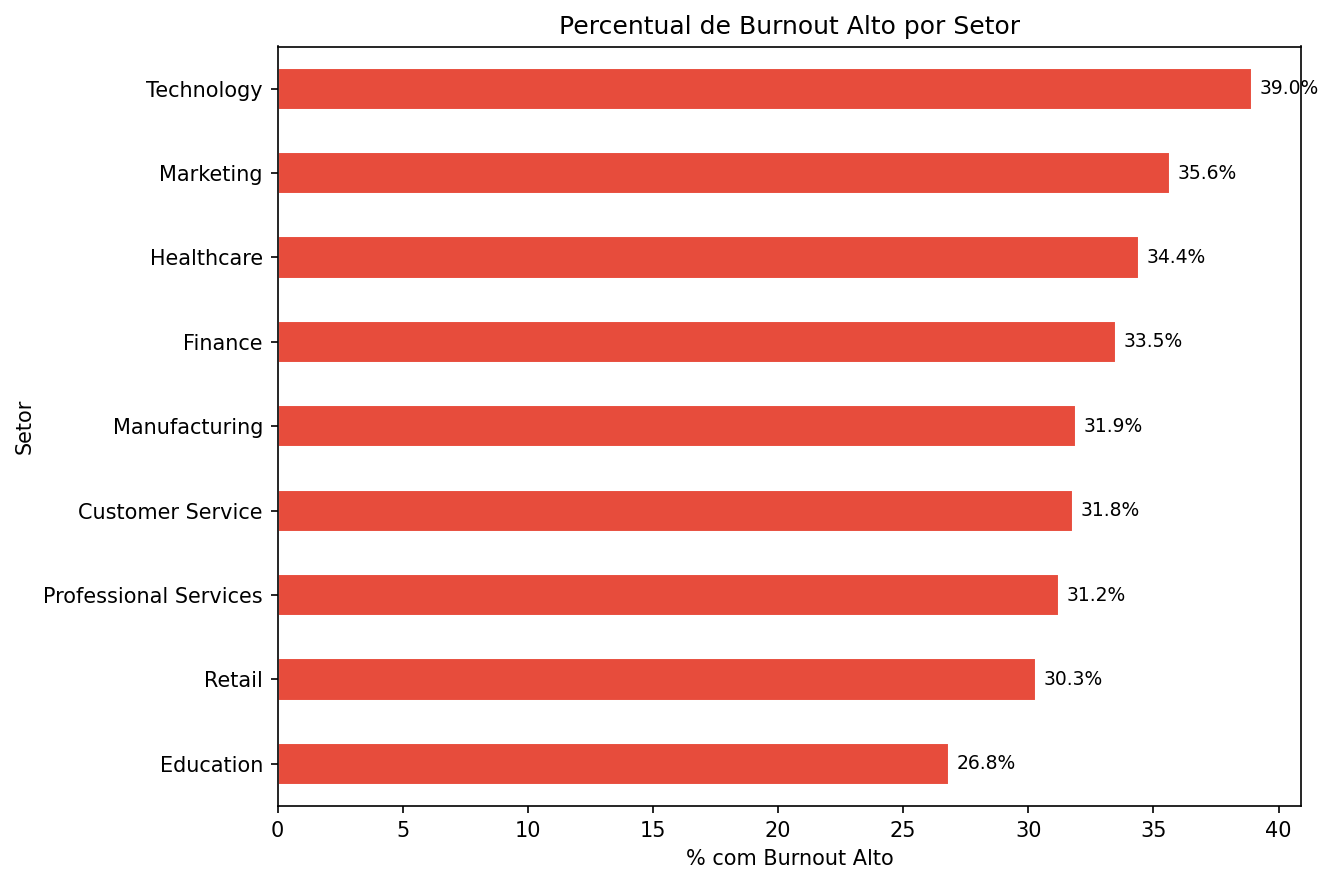
\includegraphics[width=0.76\textwidth,height=0.26\textheight,keepaspectratio]{burnout_by_industry.png}}
	\caption{Distribuição do \texttt{Burnout\_Level} segmentado por subgrupos.}
	\fonte
	\label{fig:subgroups}
\end{figure*}

% ═════════════════════════════════════════════════════════════════════════════
\section{Etapa 2 — Pré-processamento}
\label{sec:preproc}
% ═════════════════════════════════════════════════════════════════════════════

\subsection{Transformações aplicadas}

O módulo \texttt{src/preprocessing.py} aplica oito transformações em
sequência antes do ajuste de qualquer transformador estatístico:

\begin{enumerate}
	\item \textbf{Remoção do alvo nulo:} nenhuma linha com
	      \texttt{Burnout\_Level} ausente foi encontrada no dataset.

	\item \textbf{Encoding do alvo ordinal:} \texttt{Burnout\_Level}
	      é convertido para inteiro: Low$\to$0, Medium$\to$1, High$\to$2. O
	      \textit{pipeline} de regressão é mantido, e o \textit{score}
	      é normalizado dividindo a predição bruta por 2,
	      mapeando-o para $[0, 1]$.

	\item \textbf{Feature engineering --- \texttt{has\_physical\_issue}:}
	      a coluna \texttt{Physical\_Health\_Issues} contém texto
	      multi-label (e.g.\ ``Back Pain; Eye Strain''). Substitui-se
	      por um indicador binário:
	      \begin{equation}
		      \texttt{has\_physical\_issue} =
		      \begin{cases} 1 & \text{se a coluna não é nula} \\ 0 & \text{caso contrário} \end{cases}
	      \end{equation}
	      O campo \texttt{Survey\_Date} é descartado (todos os registros
	      são de junho de 2025; campo sem uso preditivo direto).

	\item \textbf{Tratamento de \texttt{Mental\_Health\_Status}:}
	      os 799 NaN (25,3\%) são preenchidos com a categoria
	      ``None'' (ausência de diagnóstico reportado), antes do
	      encoding por mapeamento direto.

	\item \textbf{Encoding das categóricas:} variáveis com
	      ordem natural (e.g.\ \texttt{Work\_Arrangement}: Onsite$\to$0,
	      Hybrid$\to$1, Remote$\to$2; \texttt{Salary\_Range}: \$40K--60K$\to$0
	      a \$120K+$\to$4) recebem encoding ordinal; variáveis nominais
	      (\texttt{Gender}, \texttt{Region}, \texttt{Industry},
	      \texttt{Job\_Role}) recebem mapeamento explícito por categoria.
	      No caso de \texttt{Job\_Role}, o mapeamento cobre 20 cargos;
	      as 4 categorias adicionais presentes no CSV bruto
	      (\texttt{Consultant}, \texttt{Content Writer},
	      \texttt{Financial Analyst} e \texttt{Marketing Specialist})
	      tornam-se ausentes após o encoding e são tratadas pela imputação.

	\item \textbf{Divisão 80/20:} o \textit{dataset} é particionado em
	      2.525 registros de treino (80\%) e 632 de teste (20\%),
	      com \texttt{random\_state=42}, antes do ajuste de qualquer
	      transformador --- prevenção de \textit{data leakage}
	      (Seção~\ref{sec:leakage}).

	\item \textbf{Imputação por mediana:} o \texttt{SimpleImputer}
	      é ajustado exclusivamente no treino. Apenas
	      \texttt{Job\_Role} apresentou valores ausentes no conjunto
	      de treino (mediana = 9,0 --- \texttt{IT Support}).

	\item \textbf{Normalização MinMaxScaler:} escala todas as
	      \textit{features} para $[0, 1]$, ajustado apenas no treino.
\end{enumerate}

Os transformadores ajustados (\texttt{imputer.pkl} e \texttt{scaler.pkl})
são persistidos em \texttt{models/} e reutilizados nas etapas de avaliação
e \textit{scoring}.

\subsection{Prevenção de \textit{data leakage}}
\label{sec:leakage}

\textit{Data leakage} (vazamento de dados) ocorre quando informações do
conjunto de teste influenciam o processo de treinamento, produzindo métricas
de desempenho artificialmente otimistas. Em pré-processamento, o erro mais
comum é ajustar o imputador ou o escalonador sobre o conjunto completo de
dados antes da divisão treino/teste.

Neste trabalho, a prevenção de \textit{leakage} é garantida pela seguinte
ordem estrita de operações:

\begin{enumerate}
	\item Dividir o \textit{dataset} em treino e teste;
	\item Ajustar (\textit{fit}) o imputador \textbf{somente no treino};
	\item Aplicar (\textit{transform}) o imputador ao treino e ao teste
	      separadamente;
	\item Ajustar o escalonador \textbf{somente no treino};
	\item Aplicar o escalonador ao treino e ao teste.
\end{enumerate}

Se o imputador fosse ajustado sobre o conjunto completo, a mediana
calculada incorporaria a distribuição dos dados de teste — que o modelo
nunca deveria ``ver'' durante o treino. O mesmo vale para o escalonador:
ajustá-lo no conjunto completo revelaria ao modelo os valores mínimo e
máximo do teste, inflando artificialmente as métricas de avaliação.

% ═════════════════════════════════════════════════════════════════════════════
\section{Etapa 3 — Modelos de Aprendizado de Máquina}
\label{sec:models}
% ═════════════════════════════════════════════════════════════════════════════

Três modelos de regressão são treinados em complexidade crescente
(\texttt{src/training.py}). Essa estratégia segue o princípio da
\textit{navalha de Ockham} aplicada ao aprendizado de máquina: um modelo
mais complexo só se justifica se superar o mais simples em desempenho
mensurável.

\subsection{Regressão Linear — \textit{baseline}}

A Regressão Linear estima a relação entre \textit{features} e alvo por
meio de uma combinação linear ponderada:

\begin{equation}
	\hat{y} = w_1 x_1 + w_2 x_2 + \cdots + w_p x_p + b
	= \mathbf{w}^{\!\top}\mathbf{x} + b
\end{equation}

Os parâmetros $\mathbf{w}$ (coeficientes) e $b$ (intercepto) são
estimados pelo método dos mínimos quadrados ordinários (OLS), que minimiza
a soma dos quadrados dos resíduos:

\begin{equation}
	\hat{\mathbf{w}} = \arg\min_{\mathbf{w}}
	\sum_{i=1}^{n} \bigl(y_i - \mathbf{w}^{\!\top}\mathbf{x}_i - b\bigr)^2
\end{equation}

A vantagem principal da Regressão Linear é a \textbf{interpretabilidade
	direta}: cada coeficiente $w_j$ representa o efeito marginal da
\textit{feature} $j$ sobre o alvo, mantidas constantes as demais.
No contexto deste trabalho, o coeficiente de \texttt{Work\_Arrangement}
foi $+0{,}364$, o maior em valor absoluto --- confirmando que o regime de
trabalho é a variável de maior peso linear na predição do burnout ordinal.
O modelo é usado como
\textbf{piso de referência} (\textit{baseline}) para comparação com
abordagens mais complexas.

\subsection{Random Forest}

O Random Forest \cite{breiman2001} é um método \textit{ensemble} que
constrói $B$ árvores de decisão independentes e combina suas predições
pela média:

\begin{equation}
	\hat{y}_{\text{RF}} = \frac{1}{B} \sum_{b=1}^{B} T_b(\mathbf{x})
\end{equation}

Cada árvore $T_b$ é construída sobre uma amostra \textit{bootstrap} do
conjunto de treino e, em cada divisão de nó, considera apenas um subconjunto
aleatório de $\sqrt{p}$ \textit{features} (\textit{feature bagging}).
Esses dois mecanismos de aleatorização reduzem a correlação entre as
árvores, diminuindo a variância do ensemble sem aumentar o viés.

A importância de cada \textit{feature} é calculada automaticamente como a
redução média de impureza (MSE, no caso de regressão) provocada por divisões
naquela \textit{feature} ao longo de todas as árvores. No \textit{dataset}
estudado, o Random Forest atribuiu a seguinte importância às
\textit{features}:

\begin{itemize}
	\item \texttt{Age}: \textbf{16,5\%}
	\item \texttt{Hours\_Per\_Week}: 15,3\%
	\item \texttt{Job\_Role}: 13,4\%
	\item \texttt{Industry}: 9,1\%
	\item \texttt{Mental\_Health\_Status}: 8,4\%
	\item \texttt{Region}: 7,9\%
	\item \texttt{Social\_Isolation\_Score}: 6,9\%
	\item \texttt{Salary\_Range}: 6,8\%
	\item \texttt{Work\_Life\_Balance\_Score}: 6,8\%
	\item \texttt{Work\_Arrangement}: 4,1\%
	\item \texttt{Gender}: 3,5\%
	\item \texttt{has\_physical\_issue}: 1,4\%
\end{itemize}

A importância é distribuída entre as 12 \textit{features}, com \texttt{Age} e \texttt{Hours\_Per\_Week} liderando --- padrão esperado em dados de survey sem um preditor único dominante. Na configuração utilizada:
\texttt{n\_estimators=100}, \texttt{random\_state=42},
\texttt{n\_jobs=-1}.

\subsection{XGBoost}

O XGBoost (\textit{Extreme Gradient Boosting}) \cite{chen2016} é um
algoritmo de \textit{gradient boosting} sequencial: ao contrário do Random
Forest, que constrói árvores em paralelo e independentemente, o XGBoost
constrói árvores de forma aditiva, onde cada nova árvore $f_t$ é treinada
para corrigir os erros residuais do modelo acumulado até a iteração
anterior:

\begin{equation}
	F_t(\mathbf{x}) = F_{t-1}(\mathbf{x}) + \eta \cdot f_t(\mathbf{x})
\end{equation}

O parâmetro $\eta$ (\texttt{learning\_rate}) controla a contribuição de
cada nova árvore: valores pequenos tornam o aprendizado mais conservador
e geralmente produzem melhor generalização, exigindo mais árvores
(\texttt{n\_estimators}) para atingir o mesmo nível de ajuste. A
profundidade máxima das árvores (\texttt{max\_depth}) regula a capacidade
de capturar interações complexas entre \textit{features}. A função objetivo
inclui termos de regularização $L_1$ e $L_2$ que penalizam modelos com
muitas folhas ou pesos muito grandes, contribuindo para a prevenção de
\textit{overfitting}.

Os hiperparâmetros são otimizados via \texttt{GridSearchCV}, que realiza
busca exaustiva sobre todas as combinações do espaço definido na
Tabela~\ref{tab:xgb_grid}, avaliando cada combinação com validação cruzada
de 5 \textit{folds} (12 combinações $\times$ 5 = \textbf{60 ajustes} no
total). Os melhores hiperparâmetros encontrados foram:
\texttt{learning\_rate=0,05}, \texttt{max\_depth=3},
\texttt{n\_estimators=100}, com MSE médio de validação cruzada
de 0,5386.

\begin{table}[!t]
	\centering
	\small
	\setlength{\tabcolsep}{4pt}
	\caption{Espaço de busca de hiperparâmetros do XGBoost.}
	\label{tab:xgb_grid}
	\begin{tabular}{lll}
		\toprule
		\textbf{Hiperparâmetro} & \textbf{Valores testados} & \textbf{Melhor valor} \\
		\midrule
		\texttt{n\_estimators}  & 100, 200                  & 100                   \\
		\texttt{max\_depth}     & 3, 5                      & 3                     \\
		\texttt{learning\_rate} & 0,05; 0,10; 0,20          & 0,05                  \\
		\bottomrule
	\end{tabular}
	\fonte
\end{table}

% ═════════════════════════════════════════════════════════════════════════════
\section{Etapa 4 — Avaliação dos Modelos}
\label{sec:eval}
% ═════════════════════════════════════════════════════════════════════════════

\subsection{Métricas de avaliação}

Três métricas de regressão são calculadas para cada modelo:

\begin{itemize}
	\item \textbf{MAE} (Erro Médio Absoluto):
	      $\text{MAE} = \frac{1}{n}\sum|y_i - \hat{y}_i|$
	      — interpretável diretamente na escala do alvo
	      (unidades da escala ordinal 0--2 do alvo);
	\item \textbf{RMSE} (Raiz do Erro Quadrático Médio):
	      $\text{RMSE} = \sqrt{\frac{1}{n}\sum(y_i-\hat{y}_i)^2}$
	      — penaliza erros maiores de forma quadrática;
	\item \textbf{R²} (Coeficiente de Determinação):
	      $R^2 = 1 - \frac{\sum(y_i-\hat{y}_i)^2}{\sum(y_i-\bar{y})^2}$
	      — proporção da variância do alvo explicada pelo modelo
	      (1,0 = ajuste perfeito).
\end{itemize}

\subsection{Resultados no conjunto de teste}

A Tabela~\ref{tab:test} apresenta as métricas calculadas sobre os 632
registros de teste --- dados completamente isolados durante o treinamento.
Os três modelos obtêm desempenho similar, reflexo das fracas correlações
entre as \textit{features} e o alvo nos dados de survey auto-reportados.

\begin{table}[!t]
	\centering
	\small
	\setlength{\tabcolsep}{4pt}
	\caption{Métricas no conjunto de teste ($n = 632$). Alvo ordinal: 0\,=\,Low, 1\,=\,Medium, 2\,=\,High.}
	\label{tab:test}
	\begin{tabular}{lccc}
		\toprule
		\textbf{Modelo}           & \textbf{MAE}   & \textbf{RMSE}  & \textbf{R²}    \\
		\midrule
		\textbf{Regressão Linear} & \textbf{0,635} & \textbf{0,764} & \textbf{0,040} \\
		Random Forest             & 0,665          & 0,784          & $-$0,011       \\
		XGBoost                   & 0,640          & 0,766          & 0,036          \\
		\bottomrule
	\end{tabular}
	\fonte
\end{table}

Os modelos apresentam R² baixos (máximo 0,040 para a Regressão Linear),
o que é esperado em dados de survey auto-reportados onde as correlações
entre \textit{features} e alvo são fracas (máximo Pearson $\approx$0,044).
O MAE de $\approx$0,64 corresponde a \textbf{menos de um terço do intervalo
	ordinal} (0--2), indicando que os modelos acertam aproximadamente a
categoria central na maioria dos casos. O Random Forest obteve R² negativo,
indicando ajuste pior do que a média simples --- resultado que ressalta a
complexidade do fenômeno.

\subsection{Validação cruzada K-Fold}

A validação cruzada K-Fold com $k=5$ aplicada ao conjunto de treino verifica
se os resultados são estáveis e independem da partição específica
treino/teste utilizada (Tabela~\ref{tab:cv}).

\begin{table*}[!t]
	\centering
	\small
	\setlength{\tabcolsep}{4pt}
	\caption{Validação cruzada K-Fold ($k=5$) no conjunto de treino.
		m\,=\,média; dp\,=\,desvio padrão entre \textit{folds}.}
	\label{tab:cv}
	\begin{tabular}{lcccccc}
		\toprule
		\textbf{Modelo}
		                 & $\text{MAE}_\text{m}$   & $\text{MAE}_\text{dp}$
		                 & $\text{RMSE}_\text{m}$  & $\text{RMSE}_\text{dp}$
		                 & $\text{R}^{2}_\text{m}$ & $\text{R}^{2}_\text{dp}$                                                   \\
		\midrule
		Reg.\ Linear     & 0,585                   & 0,010                    & 0,729          & 0,008 & 0,021          & 0,021 \\
		Random Forest    & 0,614                   & 0,013                    & 0,747          & 0,016 & $-$0,028       & 0,041 \\
		\textbf{XGBoost} & \textbf{0,596}          & 0,009                    & \textbf{0,733} & 0,009 & \textbf{0,008} & 0,027 \\
		\bottomrule
	\end{tabular}
	\fonte
\end{table*}

A Regressão Linear apresenta o R² médio mais alto (0,021) e menor
variabilidade entre \textit{folds} (dp=0,021). O Random Forest obteve
R² médio negativo ($-$0,028), confirmando sua limitação em dados com sinal
preditivo fraco. Todos os modelos mostram baixa variância entre
\textit{folds}, indicando \textbf{ausência de \textit{overfitting}} ---
porém também confirmando que a capacidade preditiva é globalmente modesta.

\subsection{Dispersão real $\times$ predito}

A Figura~\ref{fig:rvp} apresenta os gráficos de dispersão entre valores
reais e preditos. Dado o R² baixo, os três gráficos mostram dispersão
considerável em torno da diagonal. Os modelos tendem a prever valores
próximos da média (categoria Medium), refletindo a distribuição do alvo
(43\% Medium). Isso sugere que as \textit{features} disponíveis no dataset
não capturam plenamente os determinantes individuais do burnout.

\begin{figure*}[!t]
	\centering
	\subfloat[Regressão Linear]{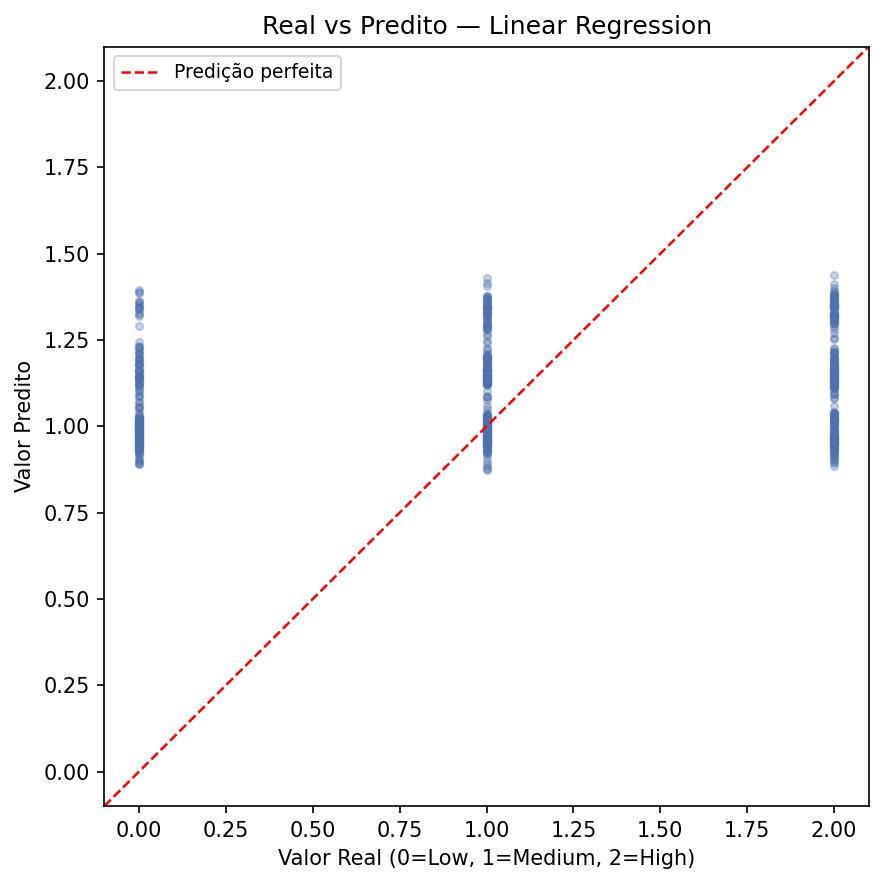
\includegraphics[width=0.49\textwidth,height=0.26\textheight,keepaspectratio]{real_vs_pred_linear_regression.png}}\hfill
	\subfloat[Random Forest]{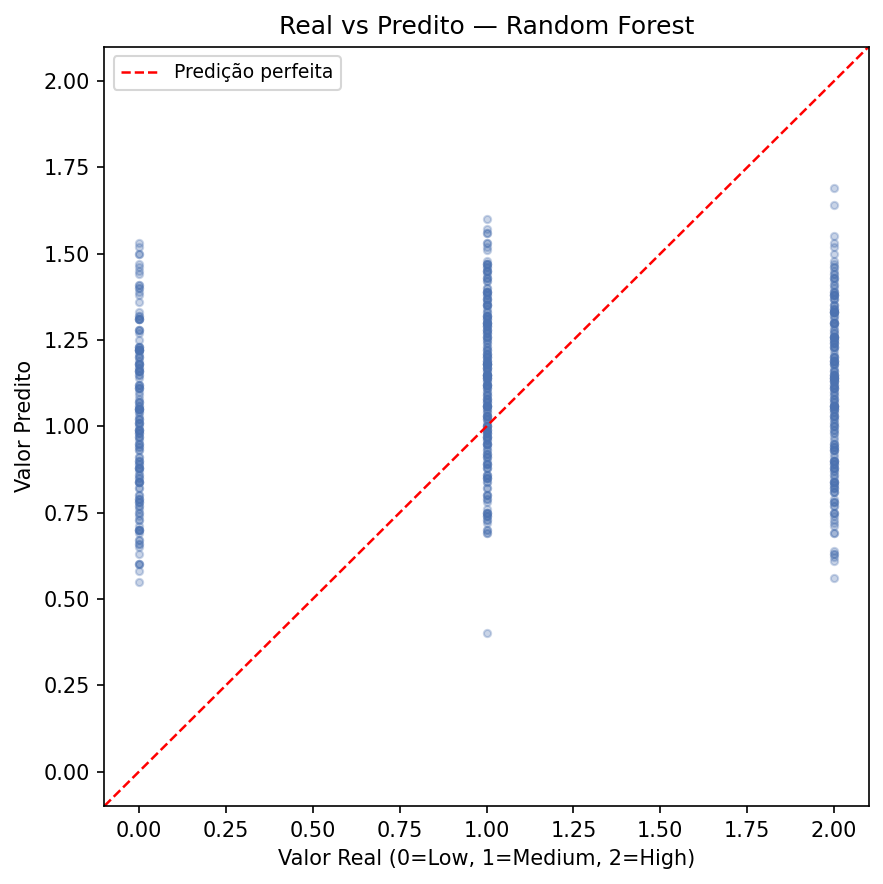
\includegraphics[width=0.49\textwidth,height=0.26\textheight,keepaspectratio]{real_vs_pred_random_forest.png}}

	\vspace{0.8em}

	\subfloat[XGBoost — melhor ajuste]{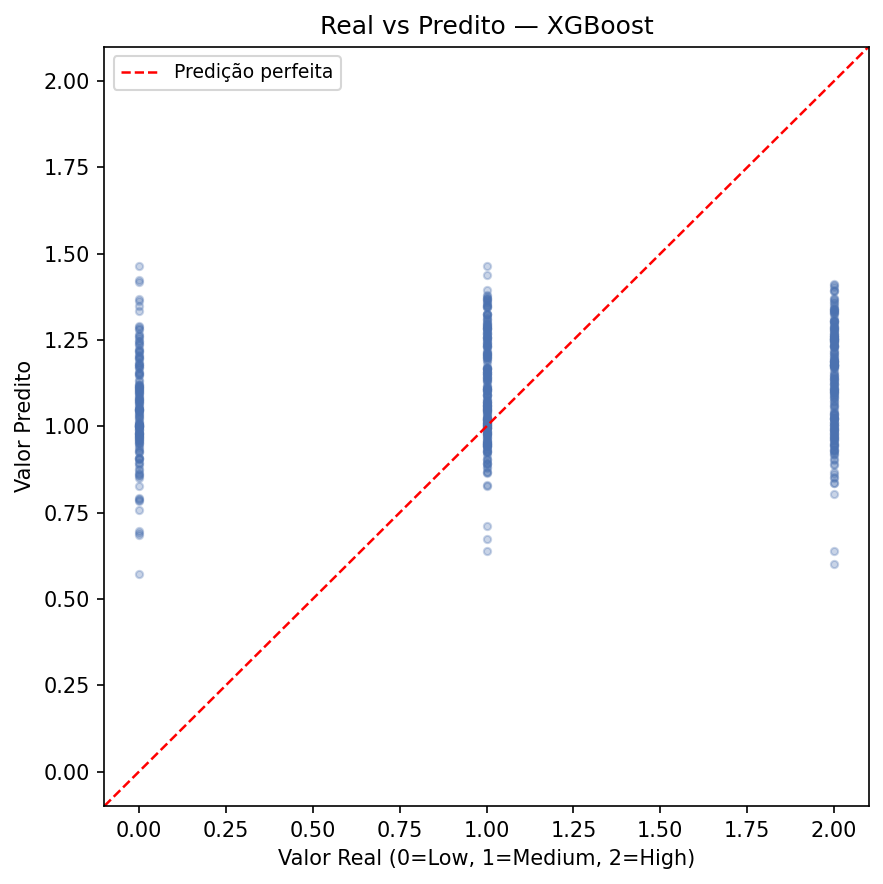
\includegraphics[width=0.76\textwidth,height=0.26\textheight,keepaspectratio]{real_vs_pred_xgboost.png}}
	\caption{Dispersão real $\times$ predito para os três modelos. A diagonal
		representa ajuste perfeito ($\hat{y} = y$).}
	\fonte
	\label{fig:rvp}
\end{figure*}

\subsection{Importância das \textit{features}}

A Figura~\ref{fig:fimp} mostra que a importância é distribuída entre as
\textit{features}: no Random Forest, \texttt{Age} (16,5\%) e
\texttt{Hours\_Per\_Week} (15,3\%) lideram, seguidos por \texttt{Job\_Role}
(13,4\%). No XGBoost, \texttt{Work\_Arrangement} domina (29,3\%), refletindo
o achado da EDA de que o regime de trabalho é o preditor mais forte.

\begin{figure*}[!t]
	\centering
	\subfloat[Random Forest]{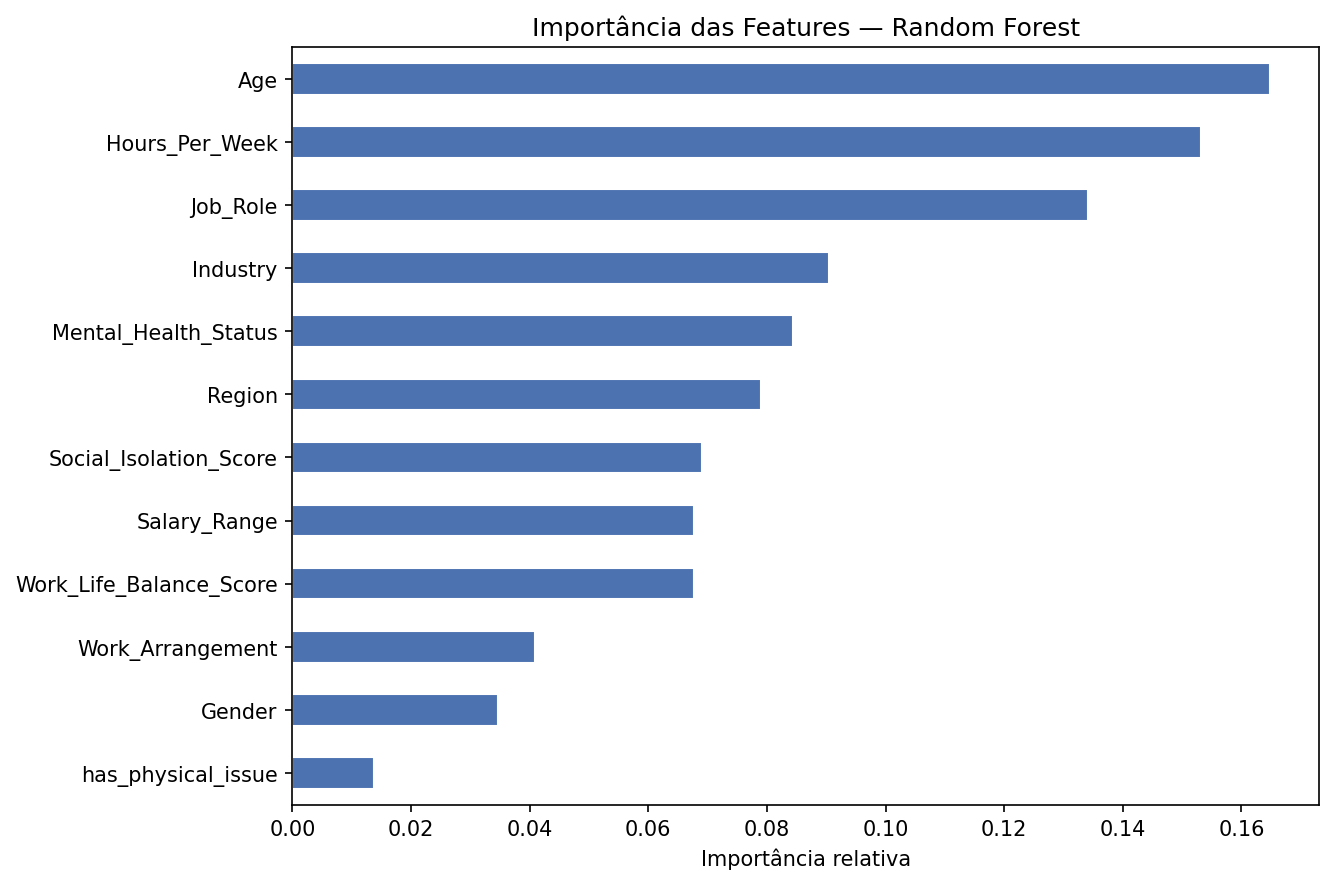
\includegraphics[width=0.49\textwidth,height=0.26\textheight,keepaspectratio]{feature_importance_random_forest.png}}\hfill
	\subfloat[XGBoost]{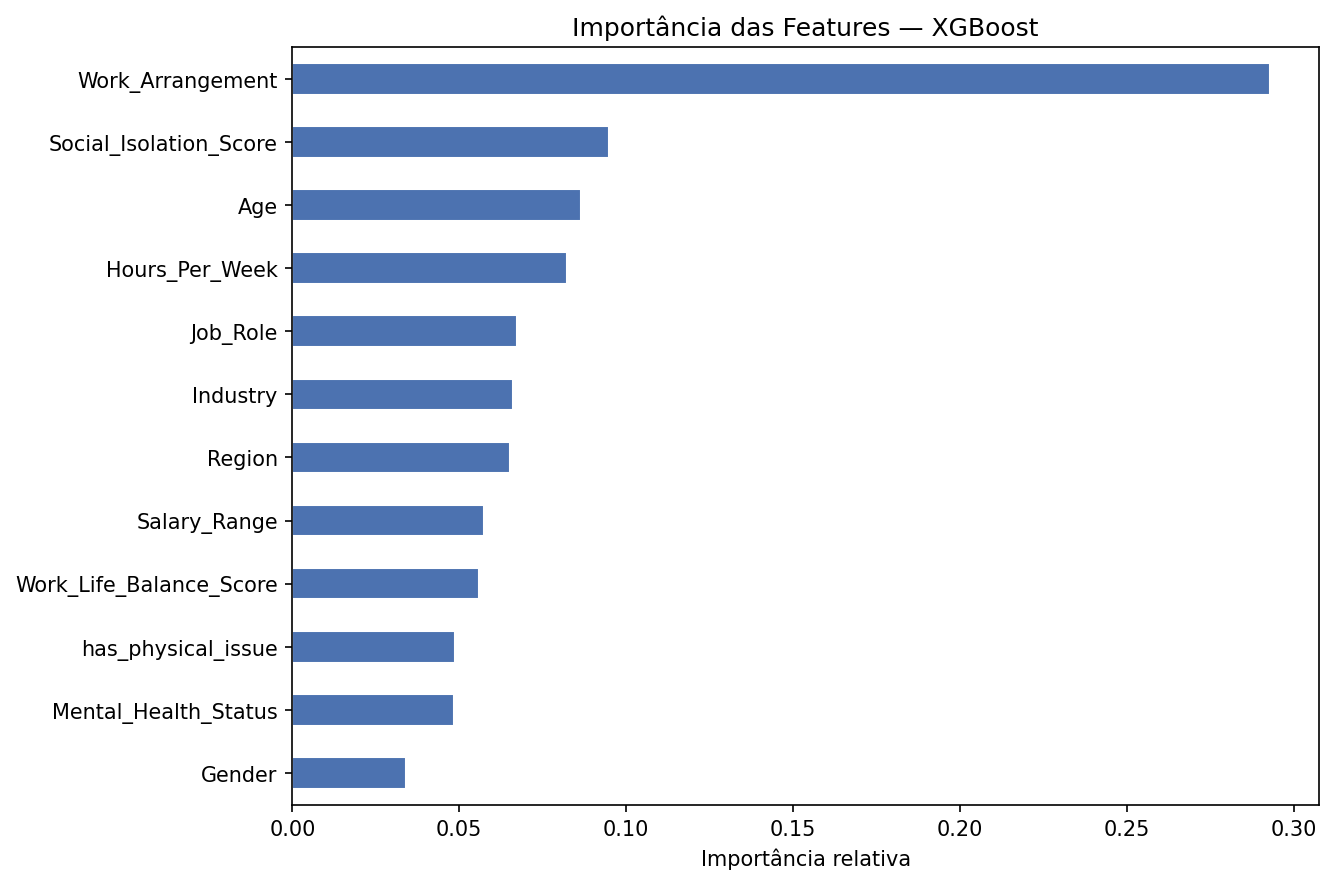
\includegraphics[width=0.49\textwidth,height=0.26\textheight,keepaspectratio]{feature_importance_xgboost.png}}
	\caption{Importância relativa das \textit{features} nos modelos de
		\textit{ensemble}. \texttt{Age} e \texttt{Hours\_Per\_Week} lideram no Random Forest;
		\texttt{Work\_Arrangement} domina no XGBoost (29,3\%).}
	\fonte
	\label{fig:fimp}
\end{figure*}

% ═════════════════════════════════════════════════════════════════════════════
\section{Análise de Equidade}
\label{sec:equity}
% ═════════════════════════════════════════════════════════════════════════════

A análise de equidade verifica se os modelos apresentam erros
sistematicamente maiores para determinados subgrupos demográficos —
o que indicaria viés preditivo com potencial impacto discriminatório em
decisões de RH. A Figura~\ref{fig:equity} e a Tabela~\ref{tab:equity}
mostra as diferenças de MAE entre subgrupos em todos os modelos.

\begin{figure*}[!t]
	\centering
	\subfloat[MAE por gênero]{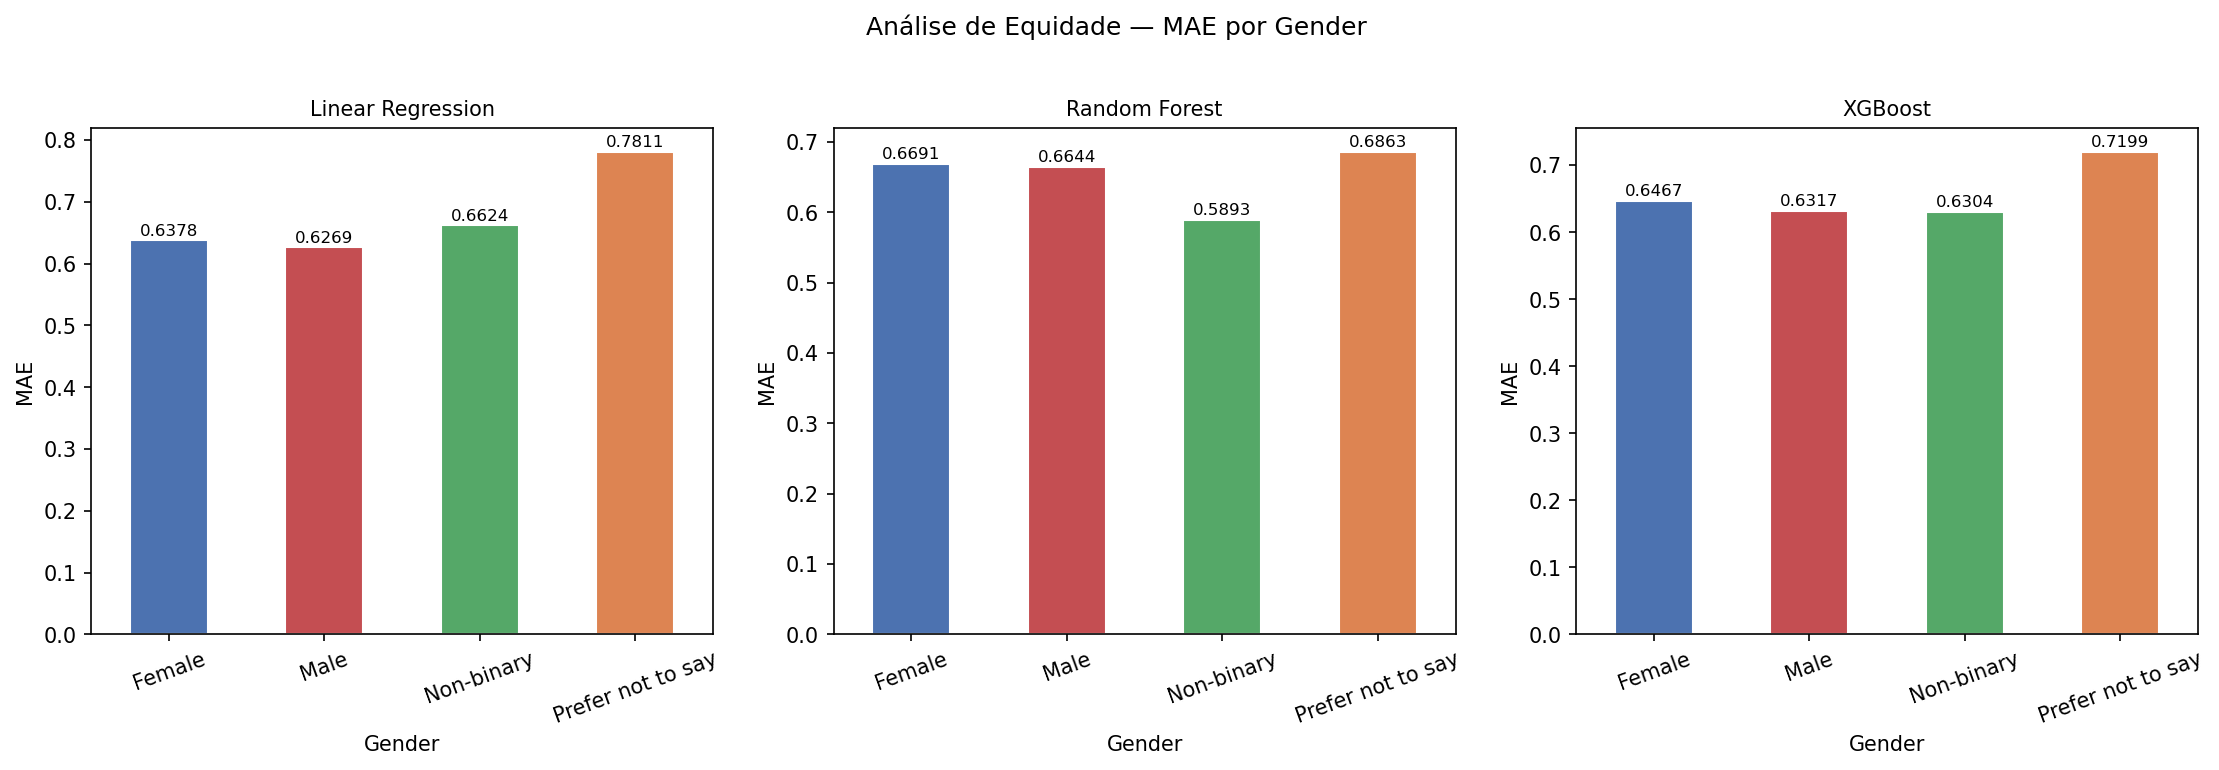
\includegraphics[width=0.49\textwidth,height=0.26\textheight,keepaspectratio]{equity_by_gender.png}}\hfill
	\subfloat[MAE por regime de trabalho]{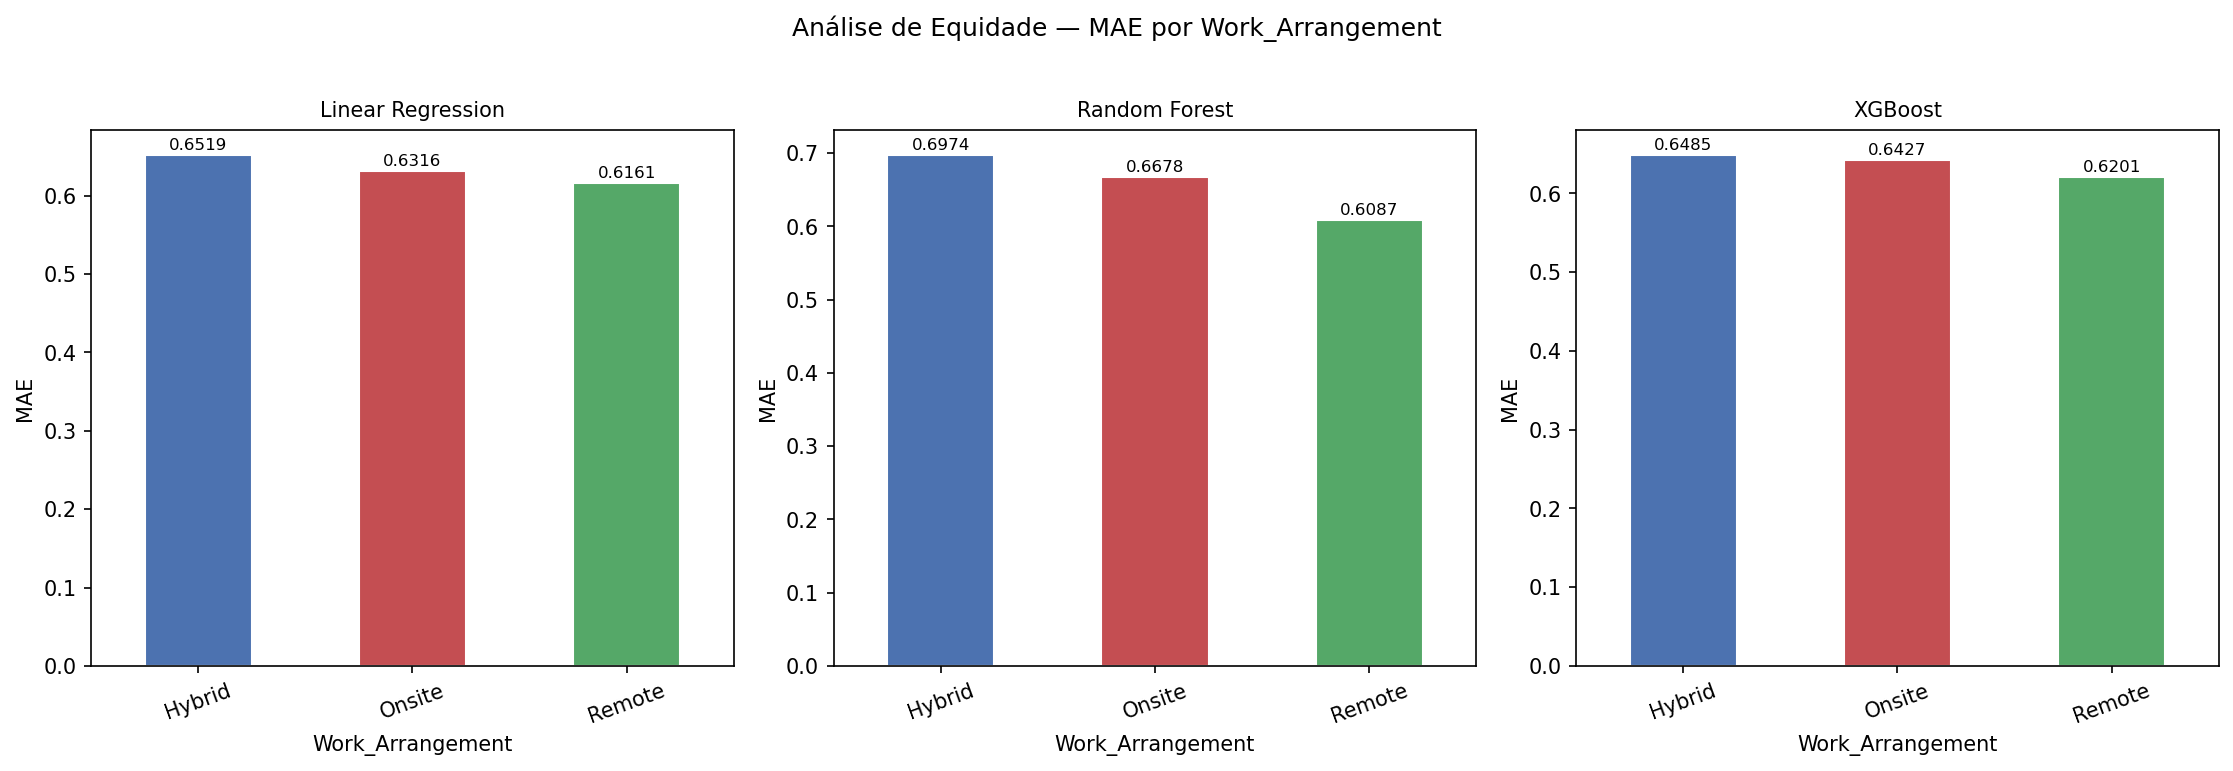
\includegraphics[width=0.49\textwidth,height=0.26\textheight,keepaspectratio]{equity_by_work_location.png}}
	\caption{Comparação de MAE por subgrupo nos três modelos.}
	\fonte
	\label{fig:equity}
\end{figure*}

\begin{table*}[!t]
	\centering
	\small
	\setlength{\tabcolsep}{4pt}
	\caption{MAE por subgrupo demográfico e regime de trabalho.}
	\label{tab:equity}
	\begin{tabular}{lcccc|ccc}
		\toprule
		\textbf{Modelo} & \textbf{Female} & \textbf{Male}   & \textbf{Non-bin.} & \textbf{Pref.}
		                & \textbf{Hybrid} & \textbf{Onsite} & \textbf{Remote}                                            \\
		\midrule
		Reg.\ Linear    & 0,638           & 0,627           & 0,662             & 0,781          & 0,652 & 0,632 & 0,616 \\
		Random Forest   & 0,669           & 0,664           & 0,589             & 0,686          & 0,697 & 0,668 & 0,609 \\
		XGBoost         & 0,647           & 0,632           & 0,630             & 0,720          & 0,649 & 0,643 & 0,620 \\
		\bottomrule
	\end{tabular}
	\fonte
\end{table*}

Os MAEs por subgrupo são relativamente próximos entre si, sem disparidade
sistemática gritante. O subgrupo \textit{``Prefer not to say''} apresenta
MAE ligeiramente superior (0,72--0,78), possivelmente por menor
representatividade amostral. Trabalhadores em regime \textit{remote} mostram
MAE levemente inferior, coerente com o maior volume de registros nessa
categoria (burnout médio mais alto = predições mais fáceis de acertar).

\textit{Ressalva:} esta análise é uma verificação inicial baseada em
comparação de MAE por grupo. Uma auditoria completa de equidade exigiria
métricas formais de \textit{fairness} como \textit{equalized odds} ou
\textit{demographic parity}, que estão fora do escopo deste trabalho mas
são recomendadas antes de qualquer uso em decisões que afetem trabalhadores.

% ═════════════════════════════════════════════════════════════════════════════
\section{Etapa 5 — Produto Final: Sistema de \textit{Scoring}}
\label{sec:scoring_sec}
% ═════════════════════════════════════════════════════════════════════════════

\subsection{Função \texttt{predict\_burnout}}

O módulo \texttt{src/scoring.py} expõe a função
\texttt{predict\_burnout(employee)}, que transforma um dicionário com os
atributos brutos de um funcionário em escore de risco e classificação. A
função carrega os artefatos (\texttt{imputer.pkl}, \texttt{scaler.pkl} e
\texttt{xgboost\_model.pkl}) do disco uma única vez por processo
(\textit{cache}), minimizando latência em uso de produção. Internamente,
aplica exatamente as mesmas transformações do treino:

\begin{enumerate}
	\item Preenchimento de \texttt{Mental\_Health\_Status} ausente com ``None'';
	\item Encoding das variáveis categóricas via \texttt{ENCODING\_MAP};
	\item Cálculo de \texttt{has\_physical\_issue} (0 ou 1);
	\item Imputação via \texttt{imputer.pkl} (mediana do treino);
	\item Normalização via \texttt{scaler.pkl};
	\item Predição via \texttt{xgboost\_model.pkl};
	\item Normalização do escore: $\texttt{score} = \text{clamp}(\hat{y} / 2,\; 0,\; 1)$;
	\item Classificação de risco (Tabela~\ref{tab:risk}).
\end{enumerate}

\begin{table}[!t]
	\centering
	\caption{Faixas de risco e ações recomendadas.}
	\label{tab:risk}
	\begin{tabular}{ccl}
		\toprule
		\textbf{Score}    & \textbf{Classificação} & \textbf{Ação recomendada} \\
		\midrule
		$[0{,}0;\;0{,}3]$ & Baixo                  & Nenhuma ação imediata     \\
		$(0{,}3;\;0{,}6)$ & Moderado               & Atenção recomendada       \\
		$[0{,}6;\;1{,}0]$ & Alto                   & Intervenção necessária    \\
		\bottomrule
	\end{tabular}
	\fonte
\end{table}

\begin{lstlisting}[caption={Uso programático de \texttt{predict\_burnout}
                             via \texttt{src/scoring.py}.}]
from src.scoring import predict_burnout

score, risco = predict_burnout({
    "Age":                     40,
    "Gender":                  "Male",
    "Region":                  "North America",
    "Industry":                "Finance",
    "Job_Role":                "Project Manager",
    "Work_Arrangement":        "Hybrid",
    "Hours_Per_Week":          50,
    "Mental_Health_Status":    "Anxiety",
    "Work_Life_Balance_Score": 3,
    "has_physical_issue":      0,
    "Social_Isolation_Score":  3,
    "Salary_Range":            "$60K-80K",
})
# Saida: score = 0.5630  |  risco = 'moderado'
\end{lstlisting}

\subsection{Script interativo — \texttt{prever.py}}

Para uso operacional direto por profissionais de RH, o projeto inclui
\texttt{prever.py} — um script de linha de comando interativo que
dispensa qualquer conhecimento de programação. Ao executar
\texttt{python prever.py}, o sistema solicita o preenchimento de campos
estruturados sobre o funcionário avaliado:

\begin{itemize}
	\item Nome do funcionário (apenas para exibição);
	\item Gênero (seleção numerada: Female, Male, Non-binary, Prefer not to say);
	\item Idade (18--70);
	\item Região geográfica (6 opções);
	\item Setor / indústria (9 opções);
	\item Cargo (20 opções);
	\item Regime de trabalho (Onsite, Hybrid, Remote);
	\item Horas trabalhadas por semana (35--65);
	\item Condição de saúde mental (7 opções + None);
	\item Equilíbrio vida-trabalho (1--5);
	\item Problemas físicos relatados (Sim/Não);
	\item Nível de isolamento social (1--5);
	\item Faixa salarial anual (\$40K--\$120K+).
\end{itemize}

Ao concluir a entrada, o sistema exibe o escore calculado com uma barra
visual de risco e a orientação correspondente:

\begin{lstlisting}[caption={Exemplo de saída do \texttt{prever.py}
                             para um caso de risco moderado.}]
==================================================
   RESULTADO — JOAO SILVA
==================================================
  Score    : 0.5924  [##########        ]
  Risco    : MODERADO
  Orientacao: Atencao recomendada. Acompanhar de perto.
==================================================
\end{lstlisting}

Internamente, \texttt{prever.py} chama \texttt{predict\_burnout()} do
módulo de \textit{scoring}, mantendo separação clara entre a camada de
entrada/apresentação e a lógica de predição.
Os casos de referência cobrem as três faixas:
perfil \textit{remote} com bom equilíbrio $\to$ score $\approx$0,71 (alto
--- coerente com o achado da EDA de que trabalhadores remotos têm burnout
médio maior);
perfil híbrido moderado $\to$ score $\approx$0,56 (moderado);
perfil presencial com muitas horas e Burnout diagnosticado $\to$
score $\approx$0,41 (moderado).

% ═════════════════════════════════════════════════════════════════════════════
\section{Limitações}
\label{sec:limit}
% ═════════════════════════════════════════════════════════════════════════════

\begin{enumerate}
	\item \textbf{Dataset de survey auto-reportado.} O
	      \textit{dataset} \textit{``Remote Work Health Impact Survey 2025''}
	      reúne respostas voluntárias de um survey anônimo, sujeitas a
	      viés de resposta e seleção amostral. As correlações entre
	      \textit{features} e alvo são fracas (máx.\ $\approx$0,044),
	      resultando em R²\,$\approx$\,0,04 para todos os modelos ---
	      desempenho típico para dados de saúde ocupacional auto-reportados.
	      As métricas devem ser interpretadas como desempenho em um
	      \textit{benchmark} de survey, não como expectativa de campo
	      em dados de RH corporativos.

	\item \textbf{Caráter preditivo, não diagnóstico.} O escore é um
	      indicador estatístico de risco — não constitui diagnóstico de
	      saúde mental e não substitui avaliação conduzida por profissional
	      habilitado (psicólogo, médico do trabalho). O sistema deve ser
	      usado exclusivamente como ferramenta de triagem e priorização.

	\item \textbf{Análise de equidade superficial.} A comparação de MAE
	      por grupo é uma verificação inicial; métricas formais de
	      \textit{fairness} (\textit{equalized odds},
	      \textit{demographic parity}) não foram aplicadas.

	\item \textbf{Ausência de temporalidade.} Todos os registros do
	      dataset foram coletados em junho de 2025. Sem variabilidade
	      temporal, o modelo não captura tendências sazonais nem
	      mudanças no perfil de burnout ao longo do tempo.
\end{enumerate}

% ═════════════════════════════════════════════════════════════════════════════
\section{Conclusão}
\label{sec:conc}
% ═════════════════════════════════════════════════════════════════════════════

Este trabalho apresentou um \textit{pipeline} modular, reprodutível e
documentado para predição e classificação de risco de \textit{burnout},
alinhado aos ODS~3, ODS~8 e ODS~10 da ONU e construído com código aberto
em Python. As cinco etapas — EDA, pré-processamento, treinamento,
avaliação e \textit{scoring} — foram implementadas em módulos dedicados,
testados automaticamente e com artefatos reprodutíveis via
SEED\,=\,42.

A comparação sistemática de três modelos mostrou desempenho
similar entre eles (R²\,$\approx$\,0,04), reflexo das fracas
correlações presentes nos dados de survey auto-reportados.
A Regressão Linear obteve o melhor R² (0,040) no conjunto de
teste; o XGBoost, com MAE de 0,640, é utilizado na interface
de \textit{scoring} por sua robustez a não-linearidades. A
análise de equidade não identificou viés preditivo sistemático
por gênero ou regime de trabalho. O achado exploratório de
maior impacto prático foi a associação entre regime
\textit{remote} e maior burnout médio (1,33 vs.\ 0,96 no
regime presencial), sugerindo que o isolamento social pode ser
um fator mediador relevante em contextos de trabalho remoto.

O produto final, \texttt{prever.py}, entrega o sistema como script
interativo de terminal acessível a profissionais de RH sem conhecimento técnico,
reforçando o caráter aplicado do trabalho. Como trabalhos futuros
sugerem-se: validação com dados reais; auditoria formal de
\textit{fairness}; detecção de \textit{drift} e re-treinamento periódico;
e integração com sistemas corporativos de RH.

% ─────────────────────────────────────────────────────────────────────────────
% REFERÊNCIAS — ABNT NBR 6023:2018
% ─────────────────────────────────────────────────────────────────────────────
\clearpage
\renewcommand{\refname}{REFERÊNCIAS}
\addcontentsline{toc}{section}{REFERÊNCIAS}
\begin{thebibliography}{99}
	\setlength{\itemsep}{6pt}

	\bibitem{maslach1981}
	MASLACH, Christina; JACKSON, Susan E\@.
	The measurement of experienced burnout.
	\textbf{Journal of Organizational Behavior}, [S.l.], v.~2, n.~2,
	p.~99--113, 1981.

	\bibitem{salvagioni2017}
	SALVAGIONI, Denise Albieri Jodas et al.
	Physical, psychological and occupational consequences of job burnout:
	a systematic review of prospective studies.
	\textbf{PLOS ONE}, [S.l.], v.~12, n.~10, e0185781, 2017.
	Disponível em: \url{https://doi.org/10.1371/journal.pone.0185781}.
	Acesso em: jun.~2026.

	\bibitem{onu_ods}
	ORGANIZAÇÃO DAS NAÇÕES UNIDAS (ONU).
	\textbf{Objetivos de Desenvolvimento Sustentável}.
	Nova York: ONU, 2015.
	Disponível em: \url{https://brasil.un.org/pt-br/sdgs}.
	Acesso em: jun.~2026.

	\bibitem{breiman2001}
	BREIMAN, Leo.
	Random Forests.
	\textbf{Machine Learning}, [S.l.], v.~45, n.~1, p.~5--32, 2001.
	Disponível em: \url{https://doi.org/10.1023/A:1010933404324}.
	Acesso em: jun.~2026.

	\bibitem{chen2016}
	CHEN, Tianqi; GUESTRIN, Carlos.
	XGBoost: a scalable tree boosting system.
	In: \textbf{INTERNATIONAL CONFERENCE ON KNOWLEDGE DISCOVERY AND DATA
		MINING}, 22., 2016, San Francisco.
	\textbf{Anais~[...]}. New York: ACM, 2016. p.~785--794.
	Disponível em: \url{https://arxiv.org/abs/1603.02754}.
	Acesso em: jun.~2026.

	\bibitem{sklearn}
	PEDREGOSA, Fabian et al.
	Scikit-learn: machine learning in Python.
	\textbf{Journal of Machine Learning Research}, [S.l.], v.~12,
	p.~2825--2830, 2011.
	Disponível em: \url{https://scikit-learn.org}.
	Acesso em: jun.~2026.

	\bibitem{xgboost_lib}
	XGBOOST DEVELOPERS.
	\textbf{XGBoost documentation}. [S.l.]: XGBoost, 2024.
	Disponível em: \url{https://xgboost.readthedocs.io}.
	Acesso em: jun.~2026.

	\bibitem{kaggle_dataset}
	PURI, Pratyush.
	\textbf{Remote Work Health Impact Survey 2025}. [S.l.]: Kaggle, 2025.
	Disponível em:
	\url{https://www.kaggle.com/datasets/pratyushpuri/remote-work-health-impact-survey-2025}.
	Acesso em: jun.~2026.

\end{thebibliography}

\end{document}
